\chapter{Modellazione e sviluppo dell'ontologia}

L'ontologia è stata creata partendo da una focalizzazione sulle entità primarie.

\section{Prosumer}
Il prosumer è l'entità principale dell'ontologia, ciò che andrà a contenere le entità caratterizzanti.


\begin{figure}[!ht]
    \centering
    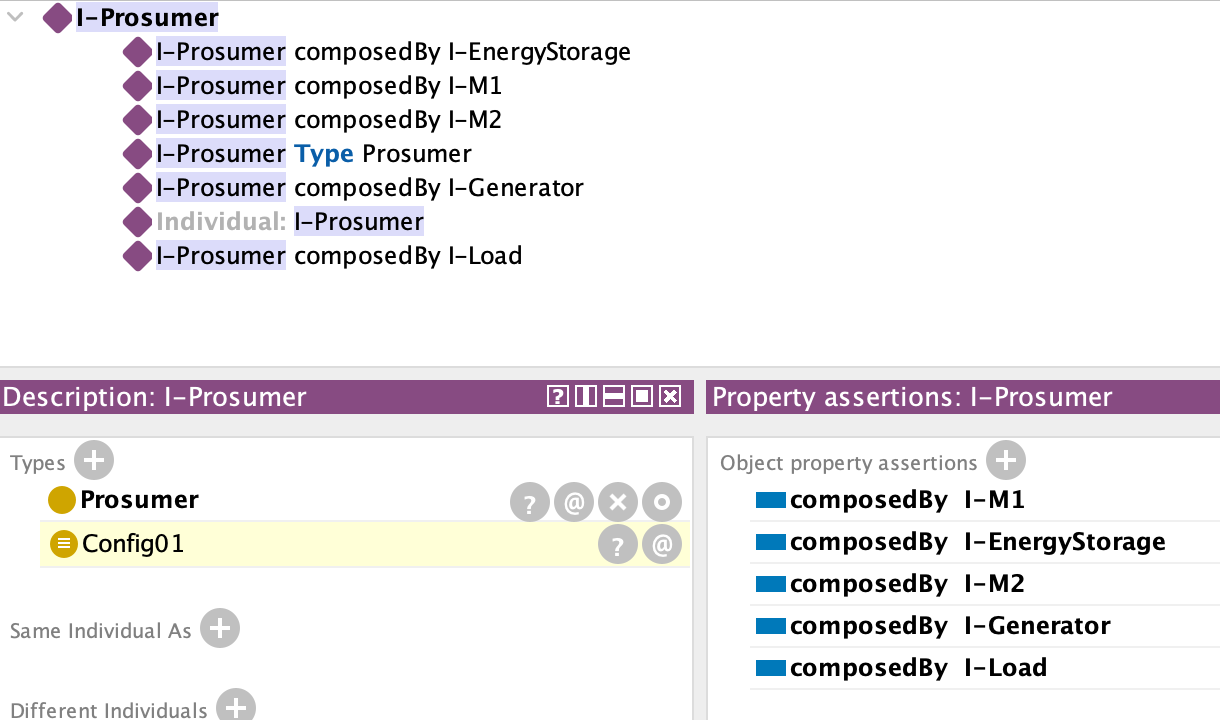
\includegraphics[width=12cm]{images/individual_prosumer.png}
    \caption{Prosumer applicato ad un individuo su Protègè.}
    \label{fig:individual_prosumer}
\end{figure}

Come si può notare nell'immagine \ref*{fig:individual_prosumer}, al prosumer vengono assegnati altri individui tramite le proprietà, grazie a ciò il reasoner è in grado di inferire la tipologia di configurazione.
In questo caso è di tipo Config01, siccome Energy Storage rispetta le caratteristiche della configurazione, come verrà mostrato nelle sezioni successive.

\subsection{Configuration}
Per stabilire la tipologia di configurazione, è stata creata la sottoclasse Configuration che a sua volta possiede le sottoclassi Config01, Config02 e Config03.

\begin{figure}[!ht]
    \centering
    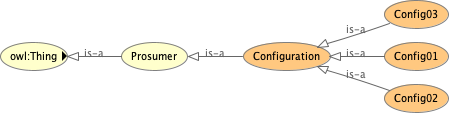
\includegraphics[width=12cm]{images/pros_graph.png}
    \caption{Grafico creato su Protègè tramite il plugin OWLViz.}
    \label{fig:pros_graph}
\end{figure}

Per specificare le caratteristiche di ogni configurazione, sono state espresse le condizioni necessarie e sufficienti. Per ogni configurazione sono presenti:
\begin{verbatim}
    Prosumer 
     and (composedBy some Generator) 
     and (composedBy some Load) 
     and (composedBy some M1) 
     and (composedBy some M2) 
\end{verbatim}

Mentre, in aggiunta per ogni configurazione:
\begin{itemize}
    \item Configurazione 01: condizioni necessarie e sufficienti: \begin{verbatim}
        and (composedBy some 
            (StorageSystem 
             and (hasDirection some Monodirectional) 
             and (hasLocation some Production) 
             and (hasPowerType some DC)))
    \end{verbatim}
          condizioni necessarie: \begin{verbatim}
        Prosumer and (not (composedBy some M3))
    \end{verbatim}
    \item Configurazione 02: condizioni necessarie e sufficienti: \begin{verbatim}
        and (composedBy some 
            (StorageSystem 
             and (hasDirection some Bidirectional) 
             and (hasLocation some Production) 
             and (hasPowerType some (AC or DC))))
    \end{verbatim}
          condizioni necessarie: \begin{verbatim}
        Prosumer and (not (composedBy some M3))
    \end{verbatim}
    \item Configurazione 03: condizioni necessarie e sufficienti \begin{verbatim}
         and (composedBy some M3) 
         and (composedBy some 
            (StorageSystem 
             and (hasDirection some Bidirectional) 
             and (hasLocation some Post-Production)
             and (hasPowerType some AC)))
    \end{verbatim}
\end{itemize}


\section{Generator}

\section{Load}

\section{Storage System}

\section{Energy Meter}


